% TODO: Do we need summaries after each subsection?
\section{Literature Review} % 2-3 Pages
In this section we will review existing literature to build an understanding of: the gestures we can expect to process, how they may be used and what they mean; Methods with which to obtain data pertaining to the pose of a head; and finally the means with which we can track movement and determine the gesture being performed.
% Types of Head Gestures (Pointing (Dietic & Manipulative) vs Semaphoric)
%   Since used by the systems mentioned in the intro, discuss these 3 types
%   Why would these types of gestures be used, what roles did they serve.
%   Examples of these gestures (with regards to systems referenced in intro)
% Probably a small section

% Head Tracking (From Smartphones)
% How track head, (Front facing camera, )
% Cascades, need face first, or one model (if using NN/ML solutions)
%   - IMU (From Head Mounted Displays and Head Mounted IMU)
%       - Will intend to use earbuds to collect IMU data of head, make footnote mentioning that this this was unfortunately not completed within this paper
%   - CNNs
%   - HAAR
%   - Alternatives (Feature extraction via histograms, etc)

% Head Gesture Recognition
% How did reviewed systems do this?
% Given data, how determine gesture performed, e.g. Dietic pointing (use raw data, e.g. calculate screen region/pointer position from data) vs Semaphoric/Manipulative classifying (given data, determine gesture performed)
%   - Derived
%   - Regression NN?
%   - RNN/LSTM (papers not specific to mobile phones)
%       - given a sequence, what class does it belong to?
%   - Markov Chain
%       - Given current state and new input, what is the new state?

% Merge last 2 sections into one?

\subsection{Gesture Classifications and Usage} % Types of Head Gesture
% Types of Head Gestures (Pointing (Dietic & Manipulative) vs Semaphoric)
%   Since used by the systems mentioned in the intro, discuss these 3 types
%   Why would these types of gestures be used, what roles did they serve.
%   Examples of these gestures (with regards to systems referenced in intro)
% Probably a small section

% Gesture classes and then discuss their examples / use-cases?
% Or
% Papers and examples, and then classification?

% Discuss why might want head gestures ?
%   - Any cases where these motions may be useful for SIIDs (Situationally Induced Impairments or Disabilities)?
% add more input options, not rely on using intuitive gestures that have since become system gestures (android navigation gestures) ~\cite{hueber2020headbang}

% Outline the types of gesture, and of those, which ones head gestures can b classified as.
% From example papers regarding head gesture control for mobile devices, look into 

Given our goal is to develop a means to distinguish head and phone gestures on smartphone devices, we first need to understand the gesture's we want to recognise and distinguish.
Here we will look at existing literature that outline the head and phone gestures you would expect to use while interfacing with a smartphone.

% Mention classes defined > mention ignore 2 as unrelated to head-gestures > explain exemplars of each type > Summary suggesting multiple employed by each system?
% Mention classes defined and list > mention ignore 2 as unrelated to head-gestures > describe several exemplars and what style/s they fit into?
% Mention classes defined and list > mention ignore 2 as unrelated to head-gestures > describe how in our review of literature that we classify as pointing/cursor manipulation vs semaphoric (gesture maps to action)
%
% https://eprints.soton.ac.uk/261149/1/GestureTaxonomyJuly21.pdf
% Breakdown the relevant gestures
After a review of gestures utilised within Human Computer Interaction literature \citeauthor{karam2005taxonomy} define five distinct classes with which we can differentiate between types of gestures utilised by the systems proposed in the literature~\cite{karam2005taxonomy}:
\begin{description}
    \item[Deictic] Gestures that involve pointing, and mapping this to either a specific object or location within the interface.
    \item[Manipulative] A gesture which indicates intent to manipulate some object.
    \item[Semaphoric] Gestures which map to a specific action or intent.
    \item[Gesticulative] Typically accompany speech, but not required to transfer meaning.
    \item[Language] A substitute to written or verbal language.
\end{description}

In our review of head/phone gesture systems we found that none utilised the Language or Gesticulative gesture styles, which is to be expected as we were focusing on gestures for control and interaction rather than for communication.
Of the 3 remaining gesture styles, we noted that systems rarely utilised a single gesture style. Either due to the gestures themselves being viewable as multiple gesture styles, being both semaphoric and manipulative, or by actively including different styles of gestures, such as pointing to a region, then using a sempahoric gesture to trigger an action.
% detail examples showing the gestures they decided upon, and why.
% example the types of gestures
% how might a phone gesture differ from head
% why might they look the same?
% yan2018headgesture, they explored existing head gestures (maybe focusing on those trackable via IMU over other methods?). Their study resulted in details shown in figure

\begin{figure}
    \centering
    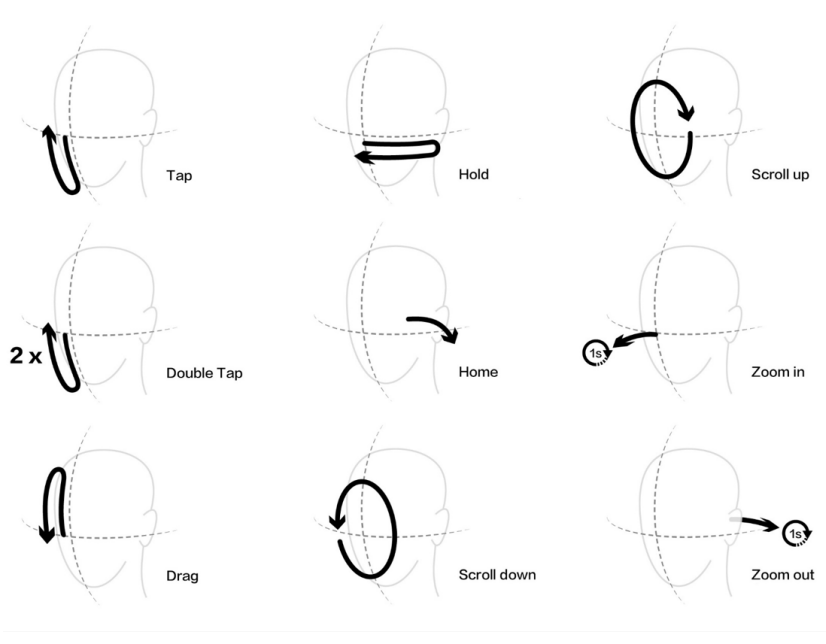
\includegraphics[width=0.5\textwidth]{figures/yan2018headgesture_fig2_proposed_gestures.png}
    \caption{\label{fig:yan2018headgesture_proposed_gestures} Proposed head gestures and their corresponding actions~\cite{yan2018headgesture}.}
    \Description[9 diagrams depicting the gestures proposed by \citeauthor{yan2018headgesture}]{9 diagrams depicitng the path of the nose taken to perform each gesture proposed by \citeauthor{yan2018headgesture}.} % TODO: Expand on this
\end{figure}

% \begin{figure*}
%     \centering
%     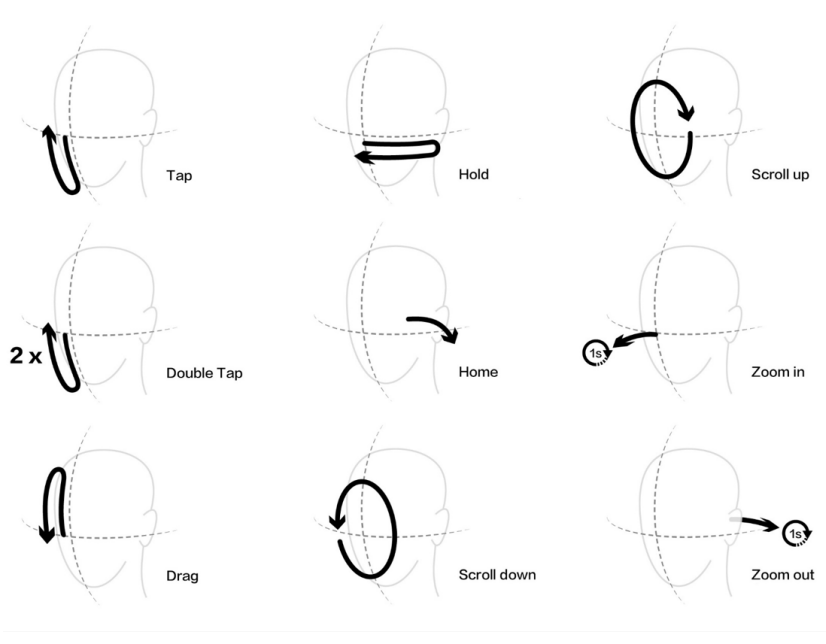
\includegraphics[width=\textwidth]{figures/yan2018headgesture_fig2_proposed_gestures.png}
%     \caption{\label{fig:yan2018headgesture_proposed_gestures} Proposed head gestures and their corresponding actions~\cite{yan2018headgesture}.}
%     \Description[9 diagrams depicting the gestures proposed by \citeauthor{yan2018headgesture}]{9 diagrams depicitng the path of the nose taken to perform each gesture proposed by \citeauthor{yan2018headgesture}.} % TODO: Expand on this
% \end{figure*}


An example of this can be seen in the work of \citeauthor{yan2018headgesture}~\cite{yan2018headgesture} who propose nine head gestures (\autoref{fig:yan2018headgesture_proposed_gestures}), the majority of which are purely Semaphoric, however several (such as scrolling, dragging, and zooming) could also be seen as Manipulative through the mapped action physically moving the content on screen.
\citeauthor{yan2018headgesture} derived these gestures through a study wherein participants where asked to proposed a set of head gestures, without being given an associated action. These gestures were then collated manually into a set of 80 gestures, which were then effectively voted upon by the participants for their respective actions.
The gestures with the most votes for a given action were selected, with some minor adjustments to ensure there were no clashes between actions.

Another system that utilised multiple gestures was EyeMu~\cite{kong2021eyemu}, which outlines several gestures that are performed by physically moving the smartphone, to improve user interaction when the user is forced to interact with phone single handed.
As with \citeauthor{yan2018headgesture}'s gestures, most are Semaphoric, but can be viewed as manipulative.
Some map to actual actions, e.g. flicking between items, others are less derivative and have less of a connection to the desired effect, e.g. moving phone closer/further from face to select an item / open a page.

% NOUSE
Two systems that were purely Deictic are Nouse~\cite{gorodnichy2004nouse} and a system developed by \citeauthor{varona2008hands}~\cite{varona2008hands}, both of which map the position of the user's nose, within images from the front-facing camera, to a location on the screen.
Neither system recognises sequences of motions of the head as gestures, other than recognising blinking and winking, which were recognised as an action to select what was under the cursor. 
You could also argue that these systems are also manipulative given they show a cursor and as such the head gestures are in an attempt to move the cursor to the relevant location.

% https://projet.liris.cnrs.fr/imagine/pub/proceedings/CVPR2012/data/papers/workshops/W01_05.pdf
One system which could be said to combine all three gesture styles would be the virtual 3D display proposed by \citeauthor{lopez2012head}~\cite{lopez2012head}.
Their system treats the smartphone screen as a window into a 3D box, visualised in \autoref{fig:lopez2012head_virtual_box}, where the region of the interior rendered is controlled via the user adjusting the position of their head with respect to the screen.
\begin{figure}
    \centering
    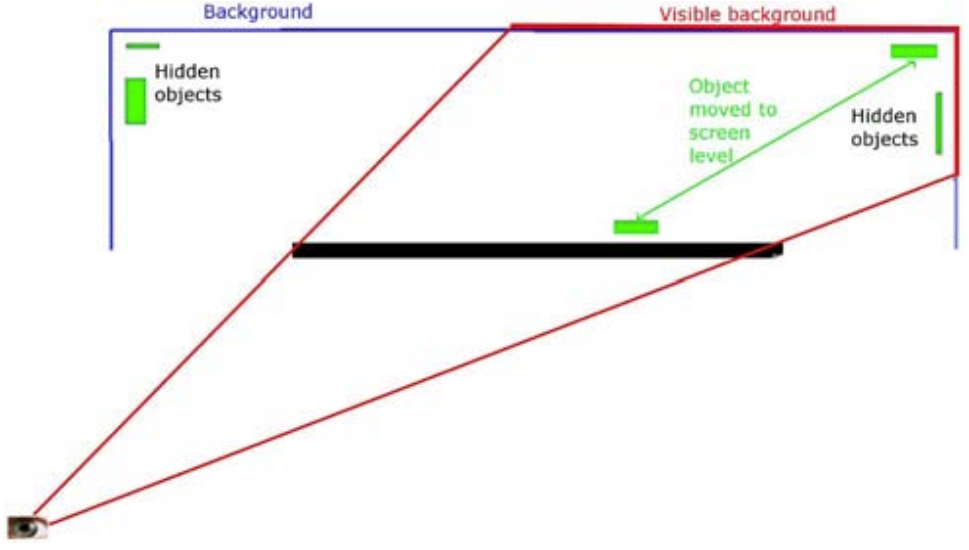
\includegraphics[width=0.45\textwidth]{figures/lopex_etal_virtual_box.png}
    \caption{\label{fig:lopez2012head_virtual_box}How user's perspective alters content that is rendered~\cite{lopez2012head}.}
    \Description{Diagram showing how a user's perspective alters content that is rendered in the app proposed by \citeauthor{lopez2012head}.} % TODO: Expand on this
\end{figure}
The tracking of relative positioning of the head to adjust the perspective of what is rendered can be seen as a form of both Deictic and Manipulative gesturing, as the user is looking at different regions within the interior of the virtual box by simply changing where they are looking, but with the intent to adjust the visible interior of the virtual box.
The system also provides Semaphoric gestures when interacting with specific programs; in one example they use a browser, with which they can look to the edge of the page to reveal the bookmarks bar.

% What conclusions can we make from this? 
% The types of gestures we expect (pointing, both manipulative and deictic, and semaphoric)

% Head bang and reach
% Initially used to 

% Phone gestures
% https://dl.acm.org/doi/pdf/10.1145/3462244.3479938

\subsection{Head Localisation}
% Image processing using front-facing camera
%   CNN (extract face position or pose/features)
%   HAAR Cascades (extract face position, or extended to features)
%   HSV Image Segmentation (extract face position, additional processing for pose etc)
%   Optical Flow (maybe extract face, or just use Optical flow to guess movement, might not need this one)
% IMU hardware (cap mounted IMU or headset)
%   Headset (not applicable)
%   Bespoke accessory with IMU, maybe use earbuds with IMU
% LIDAR/Depth Cameras (if time/space, if not, mention off-hand ignoring as not available on all devices, and not something you could buy after the fact, like headset or earbuds)
Before being able to distinguish between head and phone gestures, we first need to extract them. 
To start with we will be reviewing the methods in surrounding literature to extract relevant data required to track head gestures through the use of a smartphone.

The naive approach often taken for finding a face, or more generally a person, within an image is to perform colour segmentation~\cite{huang2004robust,bin2007rgb,chan2004face}, which involves taking an image and filtering the pixels based on a range of colour values that have been chosen as representing skin-tones.

While simple, and given favourable conditions, effective, this approach has several drawbacks:
\begin{enumerate}
    \item Detection of objects which have colours that have similar colour and chrominance levels, as noted by\citeauthor{bin2007rgb}~\cite{bin2007rgb}.
    \item Determining the values with which to segment the image, i.e. what colours will we accept as skin-tone? During their system evaluation \citeauthor{chan2004face}~\cite{chan2004face} used participants with similar skin-tones to improve the system's robustness.
    \item Dependence on environment lighting.\\
        All three of the papers above~\cite{huang2004robust,bin2007rgb,chan2004face} do make use of the HSV/yCbCr colour spaces, which make them more robust to changes in lighting intensity, however these systems can still be susceptible to changes in lighting temperature, colour, or shadows.
\end{enumerate}\nl
% \subsubsection{HAAR Cascades / The Viola Jones Algorithm}\nl
A less naive approach is the Viola-Jones algorithm proposed in 2004~\cite{viola2004robust}, used in digital cameras, smartphone camera apps, and several head gesture systems~\cite{kim2017real, neto2012real, francone2011using}.
Rather than looking for skin-tone to find faces, it uses the difference of intensity between regions of pixels, and checks if they match a set of templates, Haar-features. These features compare the relative intensity of 2, 3, or 4 neighbouring regions, e.g. is the centre of a region brighter than the regions to the left and right. 
The algorithm proposed by \citeauthor{viola2004robust} uses a degrading cascading classifier\footnote{Where a traditional cascading classifier will have possibly have 2 branches at each node, a degrading one will always exit, returning nothing, on one of the branches of each node.} to apply these Haar-features on an integral image\footnote{A representation of the input image that permits an efficient means to calculate the sum of a rectangular region of the image with just the for corner points.} and will return a bounding box for each face found.

\citeauthor{kim2017real} build upon the Viola-Jones algorithm, still utilising Haar features but building their classifier to return the locations of four facial features: left eye, right eye, nose-tip, and mouth, in place of bounding boxes~\cite{kim2017real}.

A more typical approach however is to use the Viola-Jones algorithm to retrieve the bounding box of faces within the image, and then perform further processing to extract facial features~\cite{neto2012real, francone2011using, kim2017real}.
% ~\cite{neto2012real} Also utilise HAAR-like features in a classifier, however they simply use this to identify the region of the image that contains a face, and then utilise a histogram of pixel intensity (amount of variation in a given slice of the image) to identify the eyes.
% This is done once during calibration to then extract the eyes (left eye 30\% along the line, right is 70\%) and nose (if the eyes are $d$ far apart, the nose is $d*0.45$ below the midpoint between the eyes), assuming head is upright and user is facing camera.
One downside with the algorithm that \citeauthor{viola2004robust} note is that it cannot reliably detect faces that are rotated ±15\textdegree, while the person is still facing the camera, or ±45\textdegree, where the person is facing off to the side of the camera.
% An aside on use to extract location of face, but no features
% Application of filters representing features found on common faces.
% Applied in a cascade, e.g. only check for next set of features if found large one.
% Used to reduce search space / and limit data that needs processing.

Another solution present in the literature, that is invariant to face pose, is the use of depth cameras. 
In particular we found the use of Apple's ARKit framework used alongside the front-facing depth camera (on supported iOS devices)~\cite{voelker2020headreach,hueber2020headbang,deepateep2020facial}.
ARKit provides a reliable 3D representation/positioning of the face and its features  which could be used for tracking the head's movement.
The only downside of this approach seems to be the requirement of the hardware and OS in order to use the ARKit framework.

The final solution we reviewed was the use of Convolutional Neural Networks (CNNs).
YuNet~\cite{yu2022yunet} for example outputs the bounding box along with the positions of the eyes, nose tip, and the corners of the mouth. YuNet is in fact the replacement suggested by OpenCV for detecting faces, which previously used and recommended the Viola-Jones algorithm.

\citeauthor{yan2021fast} propose a CNN which instead predicts the roll, pitch, and yaw of a face provided within an input image~\cite{yan2021fast}. With their CNN they were able to observe reduced error in their predictions compared to existing tools.

The benefit of a CNN is that they should be invariant of head rotation, given the training data includes samples of heads at different rotations.
A potential downside is the need for sufficient processing power. However there do now exist mobile variants of popular Neural Network frameworks, such as TensorFlow, with TFLite, and PyTorch, with PyTorch Mobile, which make running CNNs feasible on mobile devices.

% Android MLkit for face detection?

% Some use HAAR cascades to narrow down region
% Some alo output similar to HAAR, e.g. bounding box

\subsection{Phone Localisation}
% We now have several methods we can refer to in order to determine the head gesture being performed by a user, however we now need to explore the final area in the related works: recognising phone gestures. 
During our review of related works we came across several means of localising a smartphone / tracking a smartphone's movement, each with varying degrees of feasibility.

The least reasonable methods do not bare reviewing due to unrealistic expectations of the population of smartphone users, such as the need for a Motion Capture (MoCap) system~\cite{buschel2017investigating} or the use of a Head Mounted Display with a mounted tracking marker~\cite{mohr2019trackcap}.
These may be suitable in specific environments, but are not reasonable in meeting our goal.

A more reasonable set of methods involve localising the smartphone's position relative to its environment.
\begin{figure}
    \centering
    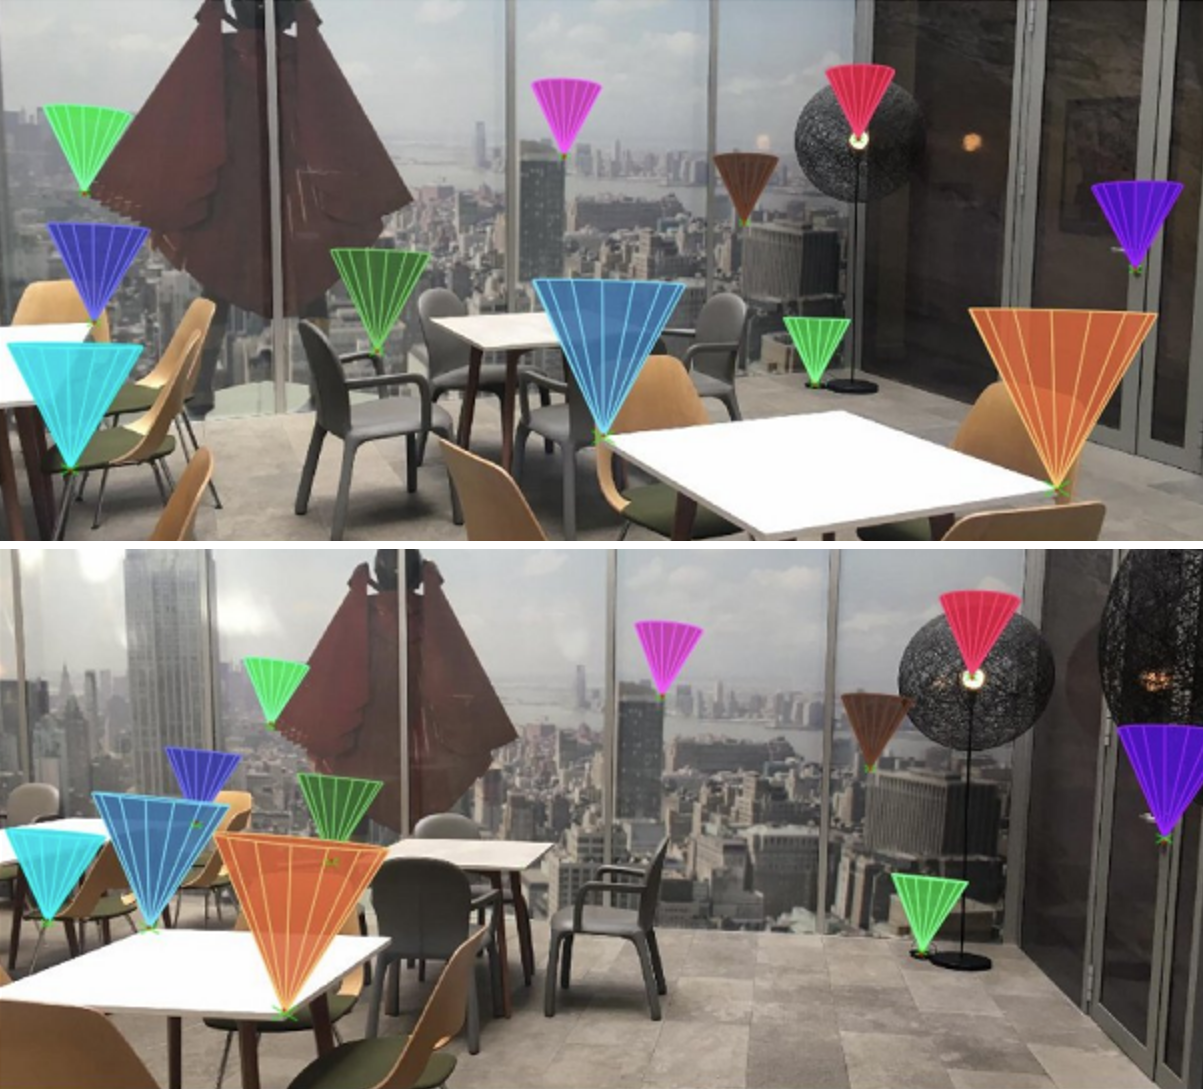
\includegraphics[width=0.45\textwidth]{figures/CameraTracking.png}
    \caption{\label{fig:barber2016camera_camera_tracking}Figure showing points being tracked~\cite{barber2016camera}.}
    \Description{Figure showing points being tracked.} % TODO: Expand on this
\end{figure}
One method is 'camera tracking', wherein the movement of the camera is estimated through analysis of an image stream from the rear-facing camera. This is a technique common-place in VFX to recreate the path taken by a camera in 3D~\cite{barber2016camera}, \autoref{fig:barber2016camera_camera_tracking} shows extracted 3D movement being used to track 3D cones into a video. However this technique has also been extended for use in Augmented Reality applications~\cite{jiang2000camera}.
Unfortunately this isn't reasonable to use on current modern mobile phones as they don't all support the ability to capture images from multiple cameras (some via software, others due to hardware limitations). As such we will not be able to utilise the rear camera as the front-camera will be required to track the user's face in our proposed system.

Another solution is the use of either Depth-Cameras or LiDaR and tracking the smartphone's movement through the observed 3D space.
Unfortunately these require special hardware that isn't available on most smartphones; most depth cameras that exist on modern smartphones are front-facing and the only current mainstream phones to provide a LiDaR on the rear of the phone are the iPhone 12 and 13 Pro series.

The only method we found to be reasonable and feasible was to record the linear and angular acceleration of a smartphone's Inertial Measurement Unit (IMU)~\cite{mantyla2000hand, kratz2013combining, neelasagar2015real, garcia2014contextualized}. 
An IMU provides the acceleration experienced in the 6 Degrees of Freedom (DoF)\footnote{3 Linear Axis: X, Y, Z, 3 Angular Axis: Yaw, Pitch, Roll} the smartphone can be manoeuvred through.
A common issue however with processing IMU output is noise, as noted by \citeauthor{neelasagar2015real}. To address potential noise they utilised low and high pass filters on the acceleration data. 

\subsection{Gesture Recognition}
% Head Gesture Recognition
% How did reviewed systems do this?
% Given data, how determine gesture performed, e.g. Dietic pointing (use raw data, e.g. calculate screen region/pointer position from data) vs Semaphoric/Manipulative classifying (given data, determine gesture performed)
%   - Derived
%   - Regression NN?
%   - RNN/LSTM (papers not specific to mobile phones)
%       - given a sequence, what class does it belong to?
%   - Markov Chain
%       - Given current state and new input, what is the new state?
Knowing how we can obtain facial features and the 'pose' of the user's head through a front-facing camera, and the localisation of the smartphone itself, the next step is to be able to recognise gestures performed by the user with either their head or the smartphone.

% \subsubsection{Relative Positioning}\nl
% NN vs Function, how best to phrase?
% Used for Pointing (Dietic)
% Great if data in is accurate (IMU may not be ideal without filtering)
One solution employed by papers proposing systems that tracked Deictic pointing gestures (and possibly Manipulative pointing gestures), was to simply use the raw data, or a function of the data, to map detected facial features to a location within the UI.

A common approach was to take the position of the nose and map it to a point on the screen. This could either be used to manipulate a cursor~\cite{gorodnichy2004nouse, varona2008hands, onuki2016combined}, allowing the user to move their head to highlight specific places on the screen, or to highlight the region of the phone the user is looking~\cite{hueber2020headbang,voelker2020headreach,roig2015face}.
% \subsubsection{Recurrent Neural Network (RNN)}\nl
% Write out the 
% Given a sequence, classify the type of motion
% not ideal if don't have known fixed number of frames, unless staggered

For semaphoric gestures you need to be able to be able to identify the gesture within a sequence of input.
An RNN is a Neural Network that takes a sequence of elements and has an internal state that is updated by some function of the current element being processed and the current state.
\citeauthor{sharma2018recognizing} proposed the use of an RNN in order to recognise head gestures, wherein the RNN input was a sequence of facial landmarks extracted from a sequence of images~\cite{sharma2018recognizing}. 
An advantage of using an RNN is that you don't strictly need to know exactly when the in the sequence the gesture was performed, just that it is present within the sequence.
A downside however is that internal state isn't maintained between predictions, as such you \textit{must} provide a sequence and the input sequence \textit{must} always be of a fixed length\footnote{This is to the best of our knowledge using common neural network frameworks such as TensorFlow and PyTorch}. Input must there for be broken-up to fixed lengths, either requiring padding prior to/after the gesture recorded (if you do not have enough elements for the required sequence). To break-up the input you need to either run the model each time-step, providing a rolling window representing the last $x$ frames of state, or to have another means to segment your recorded input to then pass into the RNN.

% \subsubsection{Hidden Markov Model (HMM)}\nl
% Given current state and new input, determine the new state
% Great if continuous input
% Another way that a Semaphoric gesture can be described is via a set of possible states, e.g. head poses or movement, and a set of rules which describe how these states can change.
Another method for predicting Semaphoric gestures from a sequence, is to use Hidden Markov Models (HMMs)~\cite{elmezain2008hidden, terven2014robust}.
A HMM describes the possible hidden states a system can be in, the probabilities/rules for transitioning from one state to another, the sates that can be observed, and the probability that a given observation arises from each hidden state.
For example, the HMM employed by \citeauthor{elmezain2008hidden}~\cite{elmezain2008hidden} has the gestures as its hidden states, in this case arabic numbers, with the possible observations being a quantised direction\footnote{To reduce the possible observation space, the angles from 0\textdegree to 360\textdegree are bucketed into a range of 0 to 18} that the user's hand travelled, captured via a camera. The probabilities of the sequence of observations would be observed for a given number drawn by the user can then be trained.

% Maybe some reinforcement learning stuff?
